\documentclass{article}
\usepackage{tabularx}
\usepackage{amsmath}
\usepackage{graphicx}
\usepackage[top = 2cm, bottom = 2cm, right = 2cm, left = 2cm]{geometry}
\usepackage{cite}
\usepackage[final]{hyperref}
\usepackage{listings}
\hypersetup{
	colorlinks=true,
	linkcolor=blue,
	citecolor=blue,
	filecolor=magenta,
	urlcolor=blue         
}

\begin{document}

\title{Practicle 2\\Raytracer - The sphere}
\date{09/01/19}
\maketitle

\begin{abstract}
	In computer graphic we need rendering technique to generate image. One of them is named the ray tracing. The aim is to send ray from the camera, intersect the 3D world and collect information for each pixel. In this practical work we'll implement a basic ray tracer to generate an image of a sphere.
\end{abstract}

\section{Introduction}
You can find on this repository some helper like a vector class and a bmp writer.
\begin{lstlisting}
	https://github.com/robinfaurypro/cuda_lessons.git
\end{lstlisting}
First, we need a buffer image. For that we can use a vector of PixelColor (you can use typedef to redefine Vector3). Each color are composed by three float. (0.f, 0.f, 0.f) is black and (1.f, 1.f, 1.f) is white. I advise you use a power of two for image resolution.

\section{Compute Capability}
Each GPU has its own property. To be more readable, Nvidia sorts GPUs with a major and a minor version. This number is named "Compute Capability". Every compute capability are registered here (https://developer.nvidia.com/cuda-gpus). After the version checking, we just have to read properties of the capability of our device. But, sometime it's possible to have multiple devices on the same PC. We can ask CUDA to list devices properties. At the beginning of your program catch the number of devices:
\begin{lstlisting}
	int nbDevices;
	cudaGetDeviceCount(&nbDevices);
\end{lstlisting}
After that, you can get properties of each device:
\begin{lstlisting}
	cudaDeviceProp prop;
	cudaGetDeviceProperties(&prop, deviceID);
	std::cout<<"Device "<<prop.name<<" | id:"<<deviceID<<std::endl;
\end{lstlisting}
Fell free to watch here (https://docs.nvidia.com/cuda/cuda-runtime-api/structcudaDeviceProp.html) all devices properties. You can find some useful values like the maxThreadsPerBlock. 

\section{Object and function in CUDA}
A usual we have to separate the host code and the device code. If you need to declare a function for the device, you just have to add the \_\_device\_\_ keyword before its signature. This keyword also work on member function.
\begin{lstlisting}
class Vector3GPU {
public:
	__device__ Vector3GPU() : x_(0.f), y_(0.f), z_(0.f) {}
	__device__ Vector3GPU(float x, float y, float z) : x_(x), y_(y), z_(z) {}
	__device__ float x() const { return x_; }
\end{lstlisting}

\section{The background}
For each feature, you have to develop a CPU fallback. The aim is to compare executions timings.\\
Before running the kernel for filling the image buffer, we need to send our vector to the global memory of the GPU. This time we'll use cudaMemcpy.
\begin{lstlisting}
Vector3* imageGPU;
cudaMalloc(&imageGPU, sizeof(Vector3)*image.size());
cudaMemcpy(imageGPU, &image[0], sizeof(Vector3)*image.size(), cudaMemcpyHostToDevice);
\end{lstlisting}
We have to be careful because this function synchronize the CPU and the GPU.\\
Next we can declare our kernel.For that, create a function with this signature:
\begin{lstlisting}
	__global__
	void clearColorGPU(Vector3* image, Vector3 backgroundColor, int w, int h)
\end{lstlisting}
Use threadIdx, blockIdx, blockDim and gridDim to find the index and the stride you need for your kernel loop. You can configure your kernel to have one thread per pixel for small resolution.
The cudaMemcpy will be used after the process to get back your buffer. (cudaMemcpyDeviceToHost)

\section{Profiling}
During the first practical we saw that we can use nvprof to profile the program. Today we'll see how using the command buffer for timings measurements. The GPU use several command buffer (one by stream). The default stream (also call the null stream) have its own FIFO command buffer. So each kernel calls are asynchronous between the device and the host, but kernels are called sequential. We can use this property to insert event marker. A cuda event is declared on the host code:
\begin{lstlisting}
	cudaEvent_t start;
	cudaEventCreate(&start);
\end{lstlisting}
After that, you just have to insert a marker before and an other after kernels, and measure the elapsed time. You may do that at the end of your program to avoid synchronization during the computation.
\begin{lstlisting}
	cudaEventRecord(start);
	kernel<<<grid, block>>>();
	cudaEventRecord(stop);
\end{lstlisting}
When you want to read the timing you should synchronize the command buffer until the event.
\begin{lstlisting}
	cudaEventSynchronize(stop);
\end{lstlisting}
Finally, get and print the value of the elapsed time gave by this CUDA function:
\begin{lstlisting}
	float milliseconds = 0;
	cudaEventElapsedTime(&milliseconds, start, stop);
\end{lstlisting}

\section{Send rays}
\begin{figure}[h]
	\centering
	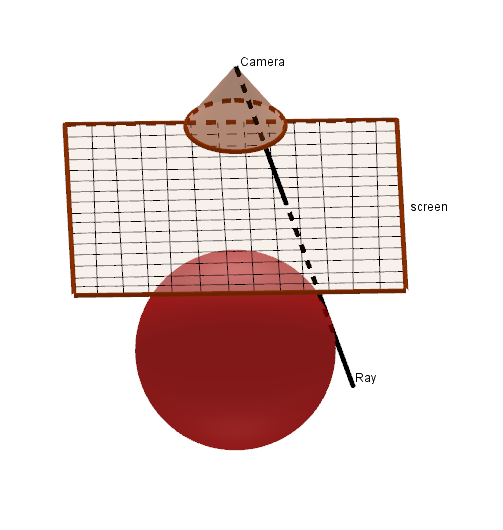
\includegraphics[scale=0.5]{figure/sendray.png}
	\caption{Send Ray}
\end{figure}
As expected, rays are the most important part of a raytracer. It's just an origin point and a direction. Create a class for instantiate a ray in a kernel and provide a function to compute a point on the ray ($P = Origin + Direction*t$).\\
Now we need a camera at the origin $(0, 0, 0)$ and a screen in front of the camera $(0, 0, -1)$. We have to choose a vertical and horizontal size of our screen in the 3D world. To avoid distortion it's a good practice to keep the same aspect ratio between your image resolution and your screen ($horizontal/vertical = width/height$). If you choose $horizontal = (2, 0, 0)$ and $vertical = (0, 2, 0)$, your lower left corner position is $(-1, -1, -1)$. With this values we can send one ray per pixel from the camera. The ray direction can be compute using this formula: $rayDir = lowerLeftCorner + (x/width)*horizontal + (y/height)*vertical$\\
For testing our program we can add an implicit surface sphere. There are a lot of algorithms to compute intersections between ray and sphere. A good C++ implementation can be found here (https://www.scratchapixel.com/lessons/3d-basic-rendering/minimal-ray-tracer-rendering-simple-shapes/ray-sphere-intersection).

\end{document}